\documentclass[a4paper]{article}

\usepackage{fullpage} % Package to use full page
\usepackage{parskip} % Package to tweak paragraph skipping
\usepackage{tikz} % Package for drawing
\usepackage{amsmath}
\usepackage{amsthm}
\usepackage{graphicx}
\usepackage{float}
\usepackage{mathtools}
\usepackage{ragged2e}
\usepackage{hyperref}
\usepackage[utf8]{inputenc}
\usepackage[ukrainian, english]{babel}
\renewcommand{\baselinestretch}{1.5}
\usepackage[T2A]{fontenc}
\usepackage[figurename=Рис.]{caption}
\usepackage[tablename=Табл.]{caption}
\renewcommand{\refname}{Література}
\addto\captionsenglish{\renewcommand{\refname}{Література}}
\addto\captionsenglish{\renewcommand{\contentsname}{Зміст}}
\renewcommand{\contentsname}{Зміст}
\newcommand\tab[1][1cm]{\hspace*{#1}}
\newcommand\norm[1]{\left\lVert#1\right\rVert}
\title{Метод скінченних елементів}
\author{Прохоров Олександр}
\date{2016}
\graphicspath{ {images/} }
\numberwithin{equation}{section}


\begin{document}
\hfill
\tableofcontents
\newpage
\section{Вступ}
Метод скінченних елементів (МСЕ) є одним з найпоширеніших методів числового розв’язування крайових задач математичної фізики. Його застосовують для розв’язування складних рiвнянь теорiї пружностi та механiки суцiльних середовищ. Процес розв’язування побудований на повному усуненні диференціального рівняння або на розкладі диференціального рівняння в часткових похід\-них в апроксимуючу систему звичайних диференціальних рівнянь.
В даній роботі розглянемо постановки крайової задачі, двоїстої до неї задачі та комплексну похибку обох задач за умови розв'язку на одній і тій же сітці.
Для розв’язування диференці\-ального рівняння використаємо метод Гальоркіна, що наближує розв’язок крайової задачі. Для покращення розв’язку будемо використовувати стратегію адаптування сітки, за допомогою апосте\-ріорного оцінювача будемо знаходити проблемні скінченні елементи. Ефективність методу покаже\-мо числовими розв’язками поставлених задач.

\section{Формулювання крайової задачі}
Розглянемо постановку крайової задачі. Необхідно знайти таку функцію $u=u(x)$ таку, що є розв’язком рівняння
\begin{equation}\label{boundaryEquation}
L[u]=f
\end{equation}
де
\begin{equation}\label{differentialOperator}
L[u]=-(\mu(x)u')'+\beta(x)u'+\sigma(x)u
\end{equation}
і задовольняє таким крайовим умовам
\begin{equation}\label{boundaryCondition}
\begin{split}
u(a)=0,\\
-\mu(b)u'(b)=\alpha[u(b)-\bar{u}].
\end{split}
\end{equation}
Тут $\mu(x)>0, \beta=\beta(x), \sigma=\sigma(x),f=f(x)$ - задані функції\\
$\alpha, \bar{u}$ - деякі сталі.
\begin{equation}
\mu \in H^1, \beta, \sigma, f\in H^0
\end{equation}
Крайова задача \ref{boundaryEquation} сформульована за допомогою лiнiйного оператора диференцiювання, який визначається у виглядi \ref{differentialOperator}.

\section{Варіаційна постановка задачі}
Знайдемо скалярний добуток лівої і правої частини рівняння з $ v \in H^1, v(a) = 0 $, де скалярний добуток має вигляд $ (u, v) = \int_a^b u(x)v(x)dx $. Тоді:
\begin{equation}
\int_a^b [-(\mu(x)u'(x))'v(x) + \beta(x)u'(x)v(x) + \sigma(x)u(x)v(x)]dx = \int_a^b f(x)v(x)dx
\end{equation}
Проінтегруємо частинами перший доданок інтегралу
\begin{equation}
-\mu(x)u'(x)v(x)\Bigr|_a^b + \int_a^b [\mu(x)u'(x)v'(x) + \beta(x)u'(x)v(x) + \sigma(x)u(x)v(x)]dx = \int_a^bf(x)v(x)dx
\end{equation}
\begin{equation}
\begin{split}
& \int_a^b [\mu(x)u'(x)v'(x) + \beta(x)u'(x)v(x) + \sigma(x)u(x)v(x)]dx \\&  - \mu(b)u'(b)v(b) + \mu(a)u'(a)v(a) = \int_a^bf(x)v(x)dx
\end{split}
\end{equation}
З умов $ v(a) = 0, -\mu(b)u'(b) = \alpha(u(b) - \bar{u}) $:
\begin{equation}
\int_a^b [\mu(x)u'(x)v'(x) + \beta(x)u'(x)v(x) + \sigma(x)u(x)v(x)]dx + \alpha u(a)v(a) = \int_a^bf(x)v(x)dx + \alpha\bar{u}v(a)
\end{equation}
Звідси запишемо білінійну форму $ a(u,v) $ і функціонал $ <l,v> $
\begin{equation}\label{variationalBilinearForm}
a(u, v) = \int_a^b [\mu(x)u'(x)v'(x) + \beta(x)u'(x)v(x) + \sigma(x)u(x)v(x)]dx + \alpha u(a)v(a)
\end{equation}
\begin{equation}\label{variationalFunctional}
<l,v> = \int_a^bf(x)v(x)dx + \alpha\bar{u}v(a)
\end{equation}
Тоді варіаційна постановка задачі матиме вигляд 
\begin{equation}\label{variationalProblem}
\begin{split}
& ? u \in H^1,
\\& a(u,v) = <l,v>, \forall v \in H^1, v(a) = 0
\end{split}
\end{equation}

Побудуємо еквівалентну задачу, яка матиме вигляд:
\begin{equation}\label{equivalentProblem}
\begin{split}
& ? u \in H^1
\\ & J(u) = \min_{ \forall v \in H^1, v(a)=0}J(v)
\end{split}
\end{equation}
де
\begin{equation}\label{equivalentEquation}
J(v) = a(u,v) - 2<l,v>
\end{equation}

\section{Побудова наближеного розв’язку}
Шукатимемо розв’язок \ref{boundaryEquation} у вигляді 
\begin{equation}\label{uhDefinition}
u_h(x)\approx\sum_{i=0}^{N} c_i\phi_i(x)
\end{equation}
де $\phi_i\in\{\phi_k\}_{k=0}^{k=N} \subset H^1. \{\phi_k\}_{k=0}^{k=N}$ - система базисних функцій розмірності N у просторі $H^1$. Підставимо $u_h$ як $u$ і $\phi_i$ як $v$ в \ref{variationalProblem}.
Отримаємо неоднорiдну систему лiнiйних алгебраїчних рiвнянь:
\begin{equation}
a(u_h, \phi_k)=<l,\phi_k>,  k=0..N
\end{equation}
\begin{equation}\label{matrixEquation}
\sum_{i=0}^{N} c_iA_{ki} = B_k,  k=0..N
\end{equation}
де
\begin{equation}\label{AkiLast}
\begin{split}
A_{ki}= \int_a^b \beta(x) \phi_i'(x) \phi_k(x) dx+
\int_a^b \sigma(x) \phi_i(x) \phi_k(x) dx + \alpha \phi_i(b) \phi_k(b)  
\end{split}
\end{equation}
\begin{equation}\label{BkLast}
B_k=\int_a^bf(x)\phi_k(x)dx + \alpha \phi_k(b) \bar{u}
\end{equation}
\begin{eqnarray}\label{equationsSystem}
\begin{bmatrix}
A_{00} & A_{01} & \cdots & A_{0N} \\
A_{10} & A_{11} & \cdots & A_{1N} \\
\vdots & \vdots & \ddots & \vdots \\
A_{N0} & A_{N1} & \cdots & A_{NN} \\
\end{bmatrix}
\begin{bmatrix}
c_0 \\
c_1 \\
\vdots \\
c_N \\
\end{bmatrix}
=
\begin{bmatrix}
B_0 \\
B_1 \\
\vdots \\
B_N \\
\end{bmatrix}
\end{eqnarray}
Розв’язавши дану систему рiвнянь отримаємо набiр коефiцiєнтiв, за допомогою яких складемо лiнiйну комбiнацiю \ref{uhDefinition}
\section{Вибір базисних функцій}
Зафіксуємо натуральне N i подiлимо вiдрiзок [a,b] на скiнченнi елементи з кроком $h=\frac{b-a}{N}$ таким чином, щоб $x_0 = a < x_1 < \ldots < x_{N-1} < x_N = b$. З наведених вище мiркувань отримаємо наступнi обмеження для системи базисних функцiй:
\begin{enumerate}
\item $\phi_i \in H^1([a, b]), i = 0, 1\ldots$
\item Для будь-якого скiнченного N система функцiй $\phi_0, \phi_1, \ldots, \phi_N$ лiнiйно незалежна на [a,b].
\item Функцiї $\phi_i, i=0,1,\ldots $ утворюють у класi $H^1([a, b])$ повну систему.
\end{enumerate}
Виберемо в якості базисних фукцій функції Куранта(кусково-лінійні поліноми першого порядку). Подамо їх в наступному вигляді:
\begin{equation}\label{courantDefinition}
\phi_i(x)=
\begin{cases} 
0, & a\leq x < x_{i-1}\\ \frac{x-x_{i-1}}{h}, & x_{i-1} < x \leq x_i\\ 
\frac{x_{i+1} - x}{h}, & x_i < x \leq x_{i+1} \\
0, & x_{i+1} < x \leq b
\end{cases}
,i=0,\ldots,N
\end{equation}
$\phi_i \in V \subset H^1([a, b]), dimV = N$. V пiдпростiр простору Соболєва в якому ми вибрали систему базисних функцiй. Якщо вибрати систему базисних функцiй таким чином, ми отримаємо тридiа\-гональну матрицю. Аналiзуючи \ref{courantDefinition} можна побачити, що iнтеграли \ref{AkiLast}, \ref{BkLast} є сенс рахувати лише на вiдповiдних скiнченних елементах.

\section{Апостеріорний оцінювач похибок}
Розглянемо наступну кусково-лінійну функцію:
\begin{equation}\label{bubbleFunctions}
b_i(x)=\begin{cases}
\frac{ x - x_i } { x_{i + \frac{1}{2} } - x_i } & \forall x \in [x_i, x_{i + \frac{1}{2}}] \\
\frac{ x_{i + 1} - x} { x_{ i + 1 } - x_{ i + \frac{1}{2} } } & \forall x \in [ x_{ i + \frac{1}{2} }, x_i] \\
\end{cases}
\end{equation}
Тут $x_{ i + \frac{1}{2} } = \frac{x_{ i + 1 } + x_i}{2}$ Шукатимемо наближення $\epsilon_h(x) \in E$ до справжньої похибки наближення $e_h~=~u-u_h$ у вигляді лінійної комбінації:
\begin{equation}
e_h(x)\approx\epsilon_h(x)=\sum_{i=0}^{N-1}\lambda_ib_i(x).
\end{equation}
Тут $\{\lambda_i\}_{i=0}^{N-1}$ - невідомі коефіцієнти. Аналогічно отримаємо схему Гальоркіна \ref{equationsSystem}, але з іншими коефцієнтами:

\begin{eqnarray}
\begin{bmatrix}
E_{00} & 0 & \cdots & 0 \\
0 & E_{11} & \cdots & 0 \\
\vdots & \vdots & \ddots & \vdots \\
0 & 0 & \cdots & E_{N-1N-1} \\
\end{bmatrix}
\begin{bmatrix}
\lambda_0 \\
\lambda_1 \\
\vdots \\
\lambda_{N-1} \\
\end{bmatrix}
=
\begin{bmatrix}
F_0 \\
F_1 \\
\vdots \\
F_{N-1} \\
\end{bmatrix}
\end{eqnarray}
де
\begin{equation}\label{Ei}
\begin{split}
E_i = ||b_i||^2 = & \int_a^b p'(x)b_i'(x)b_i(x)dx + \int_a^b p(x)b_i'(x)b_i'(x)dx + \int_a^b q(x)b_i'(x)b_i(x)dx + \\ & \int_a^b r(x)b_i(x)b_i(x)dx - p(b)b_i'(b)b_i(b) + p(a)b_i'(a)b_i(a)
\end{split}
\end{equation}
\begin{equation}\label{Fi}
\begin{split}
F_i=& <\rho(u_h),b_i>=\int_a^b f(x)b_i(x)dx-\int_a^b p'(x)u_h'(x)b_i(x)dx - \int_a^b p(x)u_h'(x)b_i'(x)dx - \\ & \int_a^b q(x)u_h'(x)b_i(x)dx - \int_a^b r(x)u_h(x)b_i(x)dx + p(b)u_h'(b)b_i(b) - p(a)u_h'(a)b_i(a)
\end{split}
\end{equation}
Коефіцієнти \ref{Ei}, \ref{Fi} отриманi шляхом замiни $u = e + u_h$ та $\phi_i = b_i$ у попереднiх кроках. Завдяки бабл-функцiї \ref{bubbleFunctions} ми отримали дiагональну проблему, з якої можна легко визначити коефiцiєнти $\lambda_i$
\begin{equation}
\lambda_i = \frac{<\rho(u_h), b_i>}{\norm{b_i}^2}
\end{equation}
\begin{equation}
\norm{e_h}^2\approx\norm{\epsilon_h}^2=\norm{\sum_{i=1}^{N-1}\lambda_ib_i}^2 = \sum_{i=1}^{N-1}\lambda_i^2\norm{b_i}^2
\end{equation}
Як бачимо з наведених міркувань, обрані базисні функції суттєво спрощують кількість обчислень для визначення похибки на кожному скінченному елементі сітки. Це може бути зручно при проектуваннi адаптивних схем МСЕ для задач бiльшої вимiрностi, де потреба локалiзацiї проблем\-них елементiв, набагато вища.

\section{Стратегія адаптування сітки}
Наведені вище вирази дають змогу побудувати рекурсивний алгоритм з допомогою якого можна згущувати сітку в місцях, де апостеріорний оцінювач визначив похибку, яка перевищує бажану точність. Таким чином на кожному скінченному елементі може бути гарантована довільна наперед задана точність. Індикатори згущення сітки визначаються таким чином:
\begin{equation}\label{error}
\eta_i=\frac{\norm{\epsilon_h}_i}{\sqrt{ \frac{1}{N} \sum_{j=0}^{N-1}(\norm{u_h}_j^2 + \norm{e_h}_j^2)}}100\%=\frac{\sqrt{N}\norm{\epsilon_h}_i} {\norm{u_h}_V^2 + \norm{e_h}_V^2} 100\%
\end{equation}
де
\begin{equation}
\norm{u_h}_i^2=\int_{x_i}^{x_{i+1}}[u_h']^2dx, u=0,\ldots, N-1
\end{equation}
Наведений вираз \ref{error} визначає, який вiдсоток становить норма похибки вiд середнього значення норми розв’язку на кожному скiнченному елементi. Якщо це число бiльше вiд заданого допустимого рiвня похибки, то цей скiнченний елемент подiляють на два новi шляхом додавання нового вузла сiтки в його центр ваги[1]. Коли ж iндикатор похибки певного скiнченного елемента не перевищує допустимого рiвня, то такий елемент без змiн входитиме до нової розрахункової сiтки. Процес згущення сітки скніченних елементів завершується за умови, що на даному кроці адаптації не було додано жодного нового вузла.
Дана стратегія дозволяє отримати розв'язок з бажаною точністю на мінімально можливій сітці.

\section{Формулювання двоїстої задача}
Двоїстою до даної називають задачу, шуканим розв'язком якої


\section{Аналiз числових результатiв}
Проведемо кілька експериментів для запропонованої схеми МСЕ і проілюструємо результати.\\
\textbf{Приклад 1.} Виберемо наступну крайову задачу:
$-u_{xx}'' + 3000(\frac{2}{3} - x)u_x'=3000, u(0)=u(1)=0$\\
Початкову сітку виберемо з 3 елементів, продемонструємо апроксимацiї розв’язку при рiзних значен\-нях N на прикладi МСЕ та адаптивного h-методу.\\
На рис.1 показано результат апроксимації використовуючи адаптивний метод згущення сітки. Апроксимація обчислена з допустимою похибкою $\delta=10\%$. Трикутниками видiлено значення у вузлах остаточної сiтки iз 63-елементiв.
\begin{figure}[H]
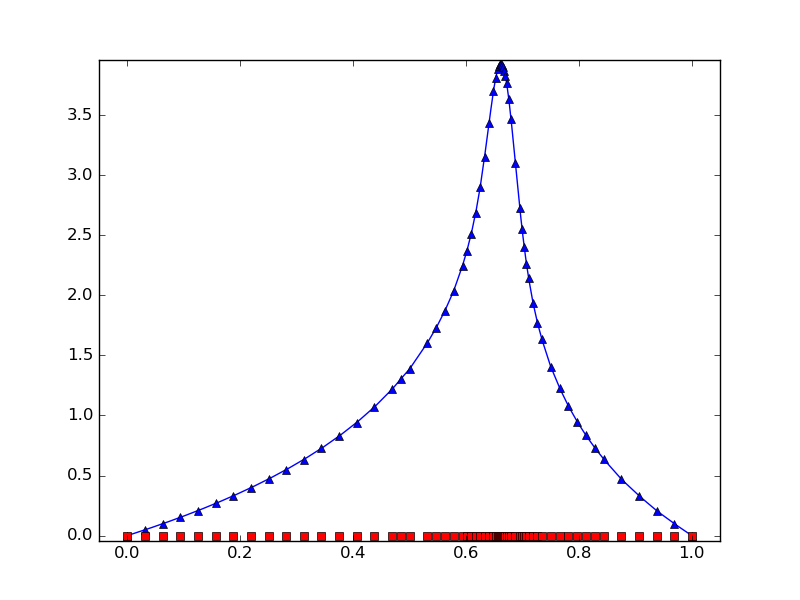
\includegraphics[width=\textwidth]{figure_1.png}
\caption{Апроксимація адаптивним методом}
\end{figure}
Табл. 1 мiстить характеристики апроксимацiї для рiвномiрно розподiленої сiтки. Як бачимо, зi збiльшенням кiлькостi елементiв $\norm{u_h}_H \to \norm{u}_H$, а $\norm{e_h}_H \to 0$. Тут
\begin{equation}
p=\ln{\frac{\norm{e_h}_{i-1}}{\norm{u_h}_i}}/\ln{\frac{N_i}{N_{i-1}}}
\end{equation}
\begin{table}[H]
\centering
\begin{tabular}{|l|l|l|l|l|l|l|l|}
\hline
N   & $||u_h||_L$ & $||e_h||_L$ & $\frac{||e_h||_L}{||u_h||_L}, \%$ & $||u_h||_H$ & $||e_h||_H$ & $\frac{||e_h||_H}{||u_h||_H}, \%$ & $p_H$    \\ \hline
10  & 1.404       & 0.51892     & 36.959                            & 11.528      & 16.178      & 140.34                            &          \\ \hline
20  & 1.3534      & 0.30873     & 22.811                            & 12.629      & 20.32       & 160.9                             & -0.32884 \\ \hline
40  & 1.3755      & 0.02358     & 1.7143                            & 12.577      & 3.1856      & 25.329                            & 2.6733   \\ \hline
80  & 1.3759      & 0.0056325   & 0.40938                           & 12.498      & 1.5414      & 12.333                            & 1.0473   \\ \hline
160 & 1.376       & 0.0013958   & 0.10144                           & 12.475      & 0.76878     & 6.1625                            & 1.0036   \\ \hline
\end{tabular}
\caption{Характеристики апроксимацiї на рiвномiрнiй сiтцi.}
\end{table}
Табл. 2 мiстить характеристики апроксимацiї для адаптивної сiтки. Можна зауважити, що на кожному кроцi N, ми отримуємо кращi значення, оскiльки значення похибки апроксимацiї зменшу\-ється. Порiвнюючи з рiвномiрно розподiленою сiткою можна побачити, що при меншiй кiлькостi елементiв ми отримаємо кращi значення апроксимацiї.

\begin{table}[H]
\centering
\begin{tabular}{|l|l|l|l|l|l|l|}
\hline
N  & $||u_h||_L$ & $||e_h||_L$ & $\frac{||e_h||_L}{||u_h||_L}, \%$ & $||u_h||_H$ & $||e_h||_H$ & $\frac{||e_h||_H}{||u_h||_H}, \%$   \\ \hline
3  & 1.7183      & 1.8556      & 107.99                            & 5.9524      & 12.856      & 215.98                                     \\ \hline
5  & 1.478       & 1.596       & 107.99                            & 7.1885      & 22.115      & 307.64                            \\ \hline
9  & 1.4503      & 1.6274      & 112.21                            & 11.144      & 45.1        & 404.69                            \\ \hline
17 & 1.3775      & 0.53343     & 38.724                            & 12.38       & 29.566      & 238.83                            \\ \hline
33 & 1.3749      & 0.037491    & 2.7269                            & 12.614      & 4.1559      & 32.947                            \\ \hline
43 & 1.376       & 0.0088723   & 0.64479                           & 12.514      & 1.9239      & 15.374                            \\ \hline
50 & 1.3762      & 0.0035187   & 0.25569                           & 12.482      & 1.0497      & 8.4097                            \\ \hline
58 & 1.3764      & 0.0024262   & 0.17627                           & 12.473      & 0.66059     & 5.2964                            \\ \hline
63 & 1.3764      & 0.0023651   & 0.17183                           & 12.471      & 0.56605     & 4.5389                            \\ \hline
\end{tabular}
\caption{Характеристики апроксимацiї на адаптивній сiтцi.}
\end{table}
\textbf{Приклад 2.} Виберемо наступну крайову задачу:
$-u_{xx}'' + 1000(1-x^7)u_x'-1000u=-1000, u(-1)=u(1)=0$\\
На рис.2 показано результат апроксимації використовуючи адаптивний метод згущення сітки. Апроксимація обчислена з допустимою похибкою $\delta=10\%$. Трикутниками видiлено значення у вузлах остаточної сiтки iз 129-елементiв.

\begin{figure}[H]
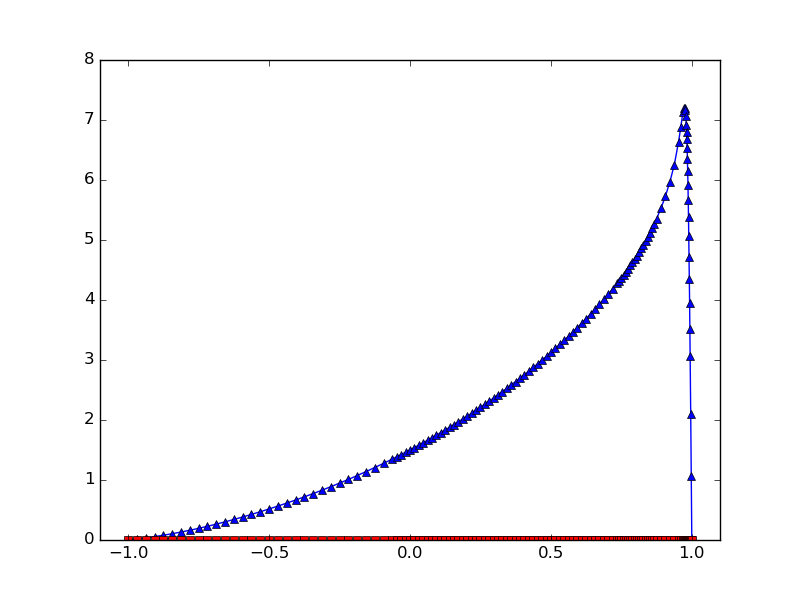
\includegraphics[width=\textwidth]{figure_2.png}
\caption{Апроксимація адаптивним методом}
\end{figure}
Табл. 3 мiстить характеристики апроксимацiї для рiвномiрно розподiленої сiтки. Як бачимо, зi збiльшенням кiлькостi елементiв, характеристики апроксимацiї покращуються.
\begin{table}[H]
\centering
\begin{tabular}{|l|l|l|l|l|l|l|l|}
\hline
N   & $||u_h||_L$ & $||e_h||_L$ & $\frac{||e_h||_L}{||u_h||_L}, \%$ & $||u_h||_H$ & $||e_h||_H$ & $\frac{||e_h||_H}{||u_h||_H}, \%$ & $p_H$   \\ \hline
10  & 1.0014      & 15.137      & 1511.7                            & 10.994      & 235.97      & 2146.3                            &         \\ \hline
20  & 1.3573      & 174.89      & 12885                             & 26.121      & 5755.6      & 22035                             & -4.6083 \\ \hline
40  & 3.3955      & 6.0979      & 179.59                            & 53.558      & 411.92      & 769.1                             & 3.8045  \\ \hline
80  & 3.7468      & 0.25431     & 6.7874                            & 55.003      & 34.798      & 63.265                            & 3.5653  \\ \hline
160 & 3.7483      & 0.041821    & 1.1157                            & 54.492      & 11.517      & 21.136                            & 1.5952  \\ \hline
\end{tabular}
\caption{Характеристики апроксимацiї на рівномірній сiтцi.}
\end{table}

Табл. 4 мiстить характеристики апроксимацiї для адаптивної сiтки. Порядок збiжностi апроксимацiї свiдчить про те, що апроксимацiя швидко збiгається до свого точного розв’язку.
\begin{table}[H]
\centering
\begin{tabular}{|l|l|l|l|l|l|l|}
\hline
N   & $||u_h||_L$ & $||e_h||_L$ & $\frac{||e_h||_L}{||u_h||_L}, \%$ & $||u_h||_H$ & $||e_h||_H$ & $\frac{||e_h||_H}{||u_h||_H}, \%$ \\ \hline
3   & 1.282       & 2.3673      & 184.66                            & 2.2205      & 8.2006      & 369.31                            \\ \hline
5   & 1.4834      & 14.864      & 1002.0                            & 4.9452      & 102.98      & 2082.4                            \\ \hline
9   & 2.1243      & 17.965      & 845.68                            & 14.817      & 248.93      & 1680.1                            \\ \hline
17  & 4.3138      & 225.45      & 5226.2                            & 54.06       & 6247.8      & 11557                             \\ \hline
32  & 2.3317      & 17.469      & 749.21                            & 51.366      & 958.35      & 1865.7                            \\ \hline
63  & 3.7584      & 3.5704      & 94.998                            & 60.109      & 293.82      & 488.81                            \\ \hline
95  & 3.7473      & 0.54565     & 14.561                            & 55.323      & 62.412      & 112.81                            \\ \hline
108 & 3.7483      & 0.065577    & 1.7495                            & 54.611      & 14.539      & 26.622                            \\ \hline
111 & 3.7497      & 0.016152    & 0.43075                           & 54.355      & 7.1286      & 13.115                            \\ \hline
115 & 3.7502      & 0.004422    & 0.11791                           & 54.28       & 3.5883      & 6.6108                            \\ \hline
122 & 3.7503      & 0.0021419   & 0.057113                          & 54.261      & 1.8564      & 3.4212                            \\ \hline
128 & 3.7503      & 0.0019789   & 0.052767                          & 54.258      & 1.3221      & 2.4367                            \\ \hline
129 & 3.7503      & 0.0019614   & 0.052301                          & 54.258      & 1.2537      & 2.3106                             \\ \hline
\end{tabular}
\caption{Характеристики апроксимацiї на адаптивній сiтцi.}
\end{table}

\newpage
\section{Висновки}
Отже, побудовано $h$-адаптивну схему МСЕ для розв’язування лiнiйних крайових задач зi звичайни\-ми диференцiальними рiвняннями другого порядку. В основі МСЕ лежить проекційний метод Галь\-оркіна, з кусково-лінійними функціями Куранта в якості базису, побудований на нерівномірній сітці скінченних елементів. Доповнено системою локального згущення сітки на проблемних скінченних елементах з використанням апостеріорного оцінювача похибки на кожному елементі, незалежно від інших. Незначні обсяги обчислень досягаються вдалим вибором ортогонального базису простору апроксимацiї похибки, а саме
вибором - кусково-лiнiйної бабл функцiї на скiнченному елементi. Запропонована $h$-адаптивна схема продемонструвала ефективнiсть в обчислювальних експеримен\-тах.
\newpage
\begin{thebibliography}{9}
\bibitem{Abramov} 
Є.Абрамов, О.Лiпiна, Г.Шинкаренко, А.Ямелець 
\textit{КУСКОВО-ЛIНIЙНI АПРОКСИМАЦIЇ h-АДАПТИВНОГО МЕТОДУ СКIНЧЕННИХ ЕЛЕМЕНТIВ ДЛЯ ОДНОВИМIРНИХ КРАЙОВИХ ЗАДАЧ}. 
ЛНУ iм. Iвана Франка, Львiв, 2006.
 
\bibitem{Strang} 
G.Strang, G.Fix
\textit{An Analysis of the Finite Element Method}. 
Wellesley-Cambridge, Wellesley, 2nd edition, 2008.

 
\bibitem{github} 
Hans Petter Langtangen Website
\\\texttt{http://hplgit.github.io/INF5620/doc/pub/main\_fem.pdf}

\bibitem{python} 
Python Homepage
\\\texttt{https://www.python.org/}


\end{thebibliography}
\end{document}